% One-page summary of the No Hesi team-driving problem set-up (batch 2, env e5). Compile with pdflatex (e.g. Overleaf).
\documentclass[10pt]{article}
\usepackage[a4paper,margin=1.15cm]{geometry}
\usepackage{amsmath,amssymb}
\usepackage{booktabs}
\usepackage{multicol}
\usepackage{enumitem}
\usepackage[dvipsnames]{xcolor}
\usepackage{tikz}
\usetikzlibrary{positioning,arrows.meta,fit}
\usepackage[hidelinks]{hyperref}
\setlength{\parindent}{0pt}
\setlength{\parskip}{1.5pt}
\setlength{\columnsep}{14pt}
\setlist{nosep,leftmargin=12pt}
\pagestyle{empty}
\newcommand{\sect}[1]{\par\smallskip{\color{MidnightBlue}\bfseries #1}\par}

\begin{document}

{\Large\bfseries Three cooperating cars on a busy highway: problem set-up}\hfill{\small batch 2, env \texttt{e5}}\\[-2pt]
\rule{\linewidth}{0.6pt}

\small
\textbf{The task.} Three team cars (BMW M3 models) drive a straight 3-lane, 10\,km highway with 20 traffic cars doing
45--60\,mph (car-following and lane changing like human drivers). Over a 120\,s episode the team scores points for
\emph{close passes} of traffic, \emph{draft passes} (passing out of a teammate's slipstream), driving as a
\emph{three-car draft train} above 80\,mph, and \emph{team passes} (all three within 40\,m); it loses points for
spreading out and for crashes (a crash wipes half the team's banked points). The question is how to drive fast and
cooperatively while never crashing.

\sect{High-level architecture: decide what to do slowly, how to do it fast}
\begin{center}
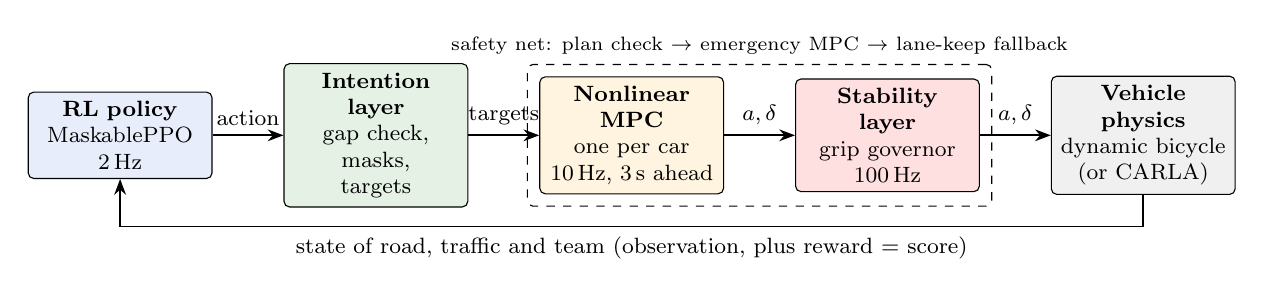
\begin{tikzpicture}[node distance=4mm and 9mm, every node/.style={font=\footnotesize},
  box/.style={draw, rounded corners=2pt, align=center, minimum height=10mm, text width=21mm, fill=#1!12},
  box/.default=gray, arr/.style={-{Stealth[length=2mm]}, semithick}]
  \node[box=RoyalBlue] (rl) {\textbf{RL policy}\\MaskablePPO\\2\,Hz};
  \node[box=ForestGreen, right=of rl] (int) {\textbf{Intention layer}\\gap check, masks,\\targets};
  \node[box=Orange, right=of int] (mpc) {\textbf{Nonlinear MPC}\\one per car\\10\,Hz, 3\,s ahead};
  \node[box=Red, right=of mpc] (stab) {\textbf{Stability layer}\\grip governor\\100\,Hz};
  \node[box=gray, right=of stab] (car) {\textbf{Vehicle physics}\\dynamic bicycle\\(or CARLA)};
  \draw[arr] (rl) -- node[above]{action} (int);
  \draw[arr] (int) -- node[above]{targets} (mpc);
  \draw[arr] (mpc) -- node[above]{$a,\delta$} (stab);
  \draw[arr] (stab) -- node[above]{$a,\delta$} (car);
  \draw[arr] (car.south) -- ++(0,-4mm) -| node[pos=0.25, below]{state of road, traffic and team (observation, plus reward = score)} (rl.south);
  \node[draw, dashed, rounded corners=2pt, fit=(mpc)(stab), inner sep=1.5mm, label={[font=\scriptsize]above:safety net: plan check $\rightarrow$ emergency MPC $\rightarrow$ lane-keep fallback}] {};
\end{tikzpicture}
\end{center}
\vspace{-2pt}
A learned \textbf{policy} picks each car's \emph{tactic} every 0.5\,s (change lane, speed up, overtake, \dots); the
\textbf{intention layer} checks it is possible (is there a gap?) and turns it into targets; a \textbf{model predictive
controller} (MPC) plans each car's steering and acceleration 3\,s ahead, every 0.1\,s, within tyre grip and clear of
other vehicles; a fast \textbf{stability layer} keeps each command within grip, like ABS and traction control.
Learning handles strategy; optimisation and physics handle safety.

\begin{multicols}{2}
\sect{1. The decision problem (what the policy learns)}
Every 0.5\,s (240 decisions per episode) the policy sees an \textbf{observation} $o_t$, picks one action per car
$a_t=(a^1_t,a^2_t,a^3_t)$, and receives a \textbf{reward} $r_t$. It is trained to maximise the expected discounted
return $\mathbb{E}\big[\sum_t \gamma^t r_t\big]$, $\gamma=0.99$ (it looks about 50\,s ahead).

\textbf{Action space} (per car, 51 discrete choices):
\begin{center}\footnotesize
\begin{tabular}{@{}lll@{}}\toprule
part & options & effect\\\midrule
lane & $-2,-1,0,+1,+2$ & two/one lanes right, keep, left\\
speed & $-1,0,+1$ & target speed $-2$\,/\,hold\,/\,$+2$\,m/s\\
lean & $-1,0,+1$ & offset 0.6\,m right\,/\,centre\,/\,left\\\midrule
overtake & right, left & pass the car ahead, then return\\
\quad margin & $+3,+6,+9$\,m/s & at least this much faster\\\bottomrule
\end{tabular}
\end{center}
$5\times3\times3=45$ lane/speed/lean combinations plus $2\times3=6$ overtakes. An overtake pulls out, passes, then
merges back in front of the passed car when there is room (else stays in the passing lane); pull-out and return follow
a smooth S-curve.

\textbf{Action masks} remove unsafe or impossible choices before the policy picks: lanes off the road; lane changes
without a gap (bumper room of 0.25\,m predicted 3\,s ahead, plus 0.3\,s per m/s a car behind closes); overtakes without
an entry gap and a clear passing lane; anything but the chosen manoeuvre while one is under way.

\textbf{Observation} (306 numbers, normalised). For each car:
\begin{itemize}
\item \emph{itself} (20): speed, sideways speed, yaw rate, steering, acceleration, offset from lane centre, heading,
lane, its manoeuvre (phase, target lane, target speed, lean, time in phase, rejected/fallback flags);
\item \emph{nearest 8 traffic cars} ($8\times7$): relative position along and across the road, relative speed,
sideways speed, present, could change lane left/right;
\item \emph{teammates} ($2\times7$): relative position and speed, their manoeuvre;
\item \emph{overtake} (11): stage (none/out/pass/return), side, passed car's relative position and speed, time,
overtake left/right possible now, return possible now;
\end{itemize}
plus 3 team values: combo multiplier, time since the last scored pass, episode time.

\textbf{Reward}: the team's score gain in that 0.5\,s (divided by 100), minus small penalties for rejected requests
($-0.1$), safety fallbacks ($-0.2$), emergency manoeuvres and unresolved conflicts ($-0.5$), aborted overtakes ($-0.1$).

\textbf{Learning}: MaskablePPO (proximal policy optimisation that respects the masks); actor and critic are
two-layer networks (256, 256, tanh); 16 simulations in parallel, 8192 decisions per update; four 5M-decision batches.
Batch 2 starts from batch 1's network (new inputs and overtake actions grafted on), learning rate $10^{-3}\to10^{-5}$,
KL limit 0.05 per update.

\sect{2. The trajectory problem (what the MPC solves)}
Each car is described in road coordinates (distance along the road $s$, offset across it $d$). The MPC state and
inputs are
\[x=[\,s,\ d,\ \psi,\ v_x,\ v_y,\ r,\ \delta,\ a\,],\qquad u=[\,\dot\delta,\ \dot a\,],\]
heading error $\psi$, body velocities $v_x,v_y$, yaw rate $r$, steering $\delta$, acceleration $a$. Every 0.1\,s it
solves, over $N=30$ steps of 0.1\,s,
\[\min_{u_0,\dots,u_{N-1}}\ \sum_{k=0}^{N}\big\|\,y_k-y^{\mathrm{ref}}_k\big\|^2_W,\]
\[y_k=[\,d_k,\ \psi_k,\ v_k,\ \delta_k,\ a_k,\ v_{y,k},\ r_k,\ \dot\delta_k,\ \dot a_k\,],\]
with $y^{\mathrm{ref}}_k$ zero except the lateral target $d^{\mathrm{ref}}_k$ and the speed target $v^{\mathrm{ref}}$
(track the target lane and speed, smoothly and without sliding), subject to: the vehicle model $x_{k+1}=f(x_k,u_k)$ (dynamic bicycle, Fiala tyres, load transfer); tyre grip (each
axle within 90\,\% of its friction circle, hard); braking $\le 0.8\,\mu g$; steering-rate and power-limited
acceleration bounds; clearance from every predicted vehicle and the road edges (soft, with a large penalty, so a
solution always exists). $d^{\mathrm{ref}}_k$ (lane centre, or the overtake S-curve) and $v^{\mathrm{ref}}$ come from
the intention layer; teammates' plans are moving obstacles. Solved with acados (real-time SQP), the first input is
applied and the problem re-solved 0.1\,s later. If a plan would still collide or exceed grip, an \emph{emergency mode}
plans brake/hold/accelerate escapes in nearby lanes; a lane-keeping law is the last resort.
\end{multicols}

\end{document}
